\documentclass{beamer}

\input{../../spec_files/course_preamble.tex}
\subtitle{Foundations of Neuro-Symbolic AI}
\date{Summer Term 2026}
\author[FONS]{Alex Goessmann}
\institute[]{
    University of Applied Science Würzburg-Schweinfurt
%    Weierstrass Institute for Applied Analysis and Stochastic
}

%\newcommand{\techwstitle}{
%\small
%%Workshop \\
%Logik für Erklärbare KI:
%Technische Einführung in das ENEXA Projekt}
%\newcommand{\smalltechwstitle}{ENEXA Workshop}

%\newcommand{\techwsdate}{15.+16. July, 2024}

%\newcommand{\techwsauthors}{
%Alex Goessmann
%}

%\newcommand{\techwsinclude}{
%	\usepackage{../../spec/beamercolorthemeclaw}
%	\usepackage{/Users/alexgoessmann/Documents/ENEXA/latex_macros/beamer_template/beamerfontthemeclaw}
%	\usepackage{/Users/alexgoessmann/Documents/ENEXA/latex_macros/beamer_template/beamerinnerthemeclaw}
%	\usepackage{/Users/alexgoessmann/Documents/ENEXA/latex_macros/beamer_template/beamerouterthemeclaw}
%
%	\input{/Users/alexgoessmann/Documents/ENEXA/latex_macros/packages.tex}
%	\input{/Users/alexgoessmann/Documents/ENEXA/latex_macros/macros.tex}
%	\input{/Users/alexgoessmann/Documents/ENEXA/latex_macros/macros_tc.tex}
%	\input{/Users/alexgoessmann/Documents/ENEXA/latex_macros/tikz_blocks.tex}
%
%	\subtitle{\techwstitle}
%	\date[\techwsdate]{\techwsdate}
%	\author[\smalltechwstitle]{\techwsauthors}
%	\institute[]{\eupic}
%}

\newcommand{\techwschapterone}{I-Tensors}
\newcommand{\techwschaptertwo}{II-Probabilities}
\newcommand{\techwschapterthree}{III-Logics}
\newcommand{\techwschapterfour}{IV-Applications}

\newcommand{\eupic}{
\begin{center}
	%\includegraphics[width=4cm]{/Users/alexgoessmann/Documents/ENEXA/latex_macros/images/fundedEU.png}
\end{center}
}

\newcommand{\enexadateveublock}{
\begin{center}\begin{tikzpicture}
  	%\node [anchor=center] at (0,0) {\includegraphics[width = 1.5cm]{/Users/alexgoessmann/Documents/ENEXA/latex_macros/images/DATEV.png}};
	%\node [anchor=center] at (2.5,0.5) {\includegraphics[width = 3.5cm]{/Users/alexgoessmann/Documents/ENEXA/latex_macros/images/enexa.png}};
	%\node [anchor=center] at (2.55,-0.5) {\includegraphics[width = 3cm]{/Users/alexgoessmann/Documents/ENEXA/latex_macros/images/fundedEU.png}};
\end{tikzpicture}\end{center}
}


%% OLD
\newcommand{\aselectionvariable}{L}
\newcommand{\vselectionvariable}{L}
\newcommand{\fselectionvariable}{L}
\newcommand{\cselectionvariable}{L}
\newcommand{\individualorder}{n}
\newcommand{\variableof}[1]{\indvariableof{#1}}
\newcommand{\sindex}{s}
\newcommand{\pindex}{p}
\newcommand{\oindex}{o}
\newcommand{\exquery}{q}
%\newcommand{\datapointof}[1]{x^{#1}}
\newcommand{\atomicqueryof}[1]{g_{#1}}
\newcommand{\facsystem}{\shortcatvariables}
\newcommand{\margprobof}[1]{\probat{#1}}
\newcommand{\mlnprobabilityof}[1]{\expdistof{#1}}
%\newcommand{\oldenexadateveublock}{
%	\begin{center}
%	\begin{minipage}{0.2\textwidth}
%		\begin{center}
%			\includegraphics[width = 2.5cm]{images/DATEV.png}
%		\end{center}
%	\end{minipage}
%	\begin{minipage}{0.55\textwidth}
%		\begin{center}
%			\includegraphics[width=5.5cm]{images/enexa.png} \\
%			\includegraphics[width=5.5cm]{images/fundedEU.png} \\
%		\end{center}
%	\end{minipage}
%	\end{center}
%}

\title[Graphical Models]{
	\techwschaptertwo \\
	{\huge Graphical Models: Representing Probabilities as Tensor Networks}
}
\begin{document}

{\frame[plain]{\titlepage}}



\begin{frame}{How to beat the curse of dimensions?}

Probability distribution of factored systems with states $\facstates$ has 
	\[\left(\prod_{\atomenumeratorin}\catdimof{\atomenumerator}\right) -1 \]
degrees of freedom (coordinates to specify and store).

\medskip

Mitigation: \emph{Tensor Network Decompositions}

\begin{block}{Independencies of Random Variables}
	Decompositions of Probability Tensors correspond with independencies of (hidden) random variables.
\end{block}

\end{frame}



\begin{frame}{Example: Being at a dentist}

Add a variable \emph{Cloud}, denoting the weather outside the dentists lab.
\begin{itemize}
	\item This adds an additional axis to $\probtensor$, thus the number of coordinates increases by a factor of $2$.
	\item But: Intuitively, knowing \emph{Cloud} should not affect the probability of having a cavity, so why shall we care?
\end{itemize}

\begin{block}{Independence of Cloud to the other Variables}
	After showing that cavity, catch and toothache are independent of cloud, we do not have to consider cloud any more.
\end{block}

\end{frame}



\begin{frame}{Formal definition of Independencies}

\begin{definition}[Independence]
	Given a joint distribution of variables $\exrandom$ and $\secexrandom$, we say that $\exrandom$ is independent from $\secexrandom$ if for any values $\catindexof{\exrandom},\catindexof{\secexrandom}$ we have
		\[ \probof{\exrandom=\catindexof{\exrandom},\secexrandom=\catindexof{\secexrandom}} 
		= \margprobof{\exrandom=\catindexof{\exrandom}}{\exrandom}
		 \cdot 
		 \margprobof{\secexrandom=\catindexof{\secexrandom}}{\secexrandom} \, . \]
\end{definition}
In the tensor network decomposition we depict this by
	\begin{center}
		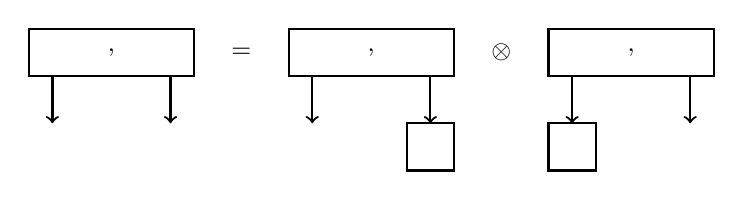
\begin{tikzpicture}[scale=0.3,thick] % , baseline = -3.5pt


\draw (0,1) rectangle (7,-1);
\node[anchor=center] (text) at (3.5,0) {\small $\probof{\exrandom,\secexrandom}$};
\draw[->] (1,-1) -- (1,-3) node[midway, left] {\tiny $\exrandom$};
\draw[->] (6,-1) -- (6,-3) node[midway, left] {\tiny $\secexrandom$};

\node[anchor=center] (text) at (9,0) {\small ${=}$};


\begin{scope}[shift={(11,0)}]

\draw (0,1) rectangle (7,-1);
\node[anchor=center] (text) at (3.5,0) {\small $\probof{\exrandom,\secexrandom}$};
\draw[->] (1,-1) -- (1,-3) node[midway, left] {\tiny $\exrandom$};
\draw[->] (6,-1) -- (6,-3) node[midway, left] {\tiny $\secexrandom$};
\draw (5,-3) rectangle (7,-5);
\node[anchor=center] (text) at (6,-4) {\small $\ones$};

\end{scope}

\node[anchor=center] (text) at (20,0) {\small $\otimes$};

\begin{scope}[shift={(22,0)}]

\draw (0,1) rectangle (7,-1);
\node[anchor=center] (text) at (3.5,0) {\small $\probof{\exrandom,\secexrandom}$};
\draw[->] (1,-1) -- (1,-3) node[midway, left] {\tiny $\exrandom$};
\draw (0,-3) rectangle (2,-5);
\node[anchor=center] (text) at (1,-4) {\small $\ones$};
\draw[->] (6,-1) -- (6,-3) node[midway, left] {\tiny $\secexrandom$};

\end{scope}


\end{tikzpicture} 
	\end{center}
\end{frame}


\begin{frame}{Contraction criterion for independence}

\begin{theorem}\label{the:independenceProductCriterion}
	Given a probability distribution $\probtensor$, $\exrandom$ is independent from $\secexrandom$, if and only if 
	\begin{align*}
		\probtensor = \contractionof{\probtensor}{\exrandom} \otimes  \contractionof{\probtensor}{\secexrandom} \, .
	\end{align*}
\end{theorem}

\end{frame}



\begin{frame}{Decomposition into Marginal Probability Tensors}
	Independence allows the decomposition into 
	\begin{center}
		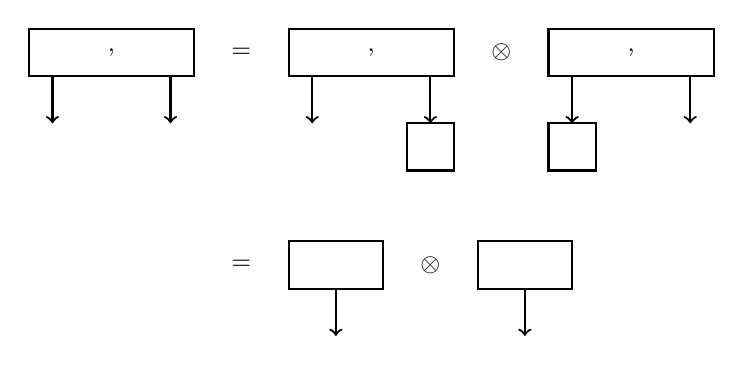
\begin{tikzpicture}[scale=0.3,thick] % , baseline = -3.5pt


\draw (0,1) rectangle (7,-1);
\node[anchor=center] (text) at (3.5,0) {\small $\probof{\exrandom,\secexrandom}$};
\draw[->] (1,-1) -- (1,-3) node[midway, left] {\tiny $\exrandom$};
\draw[->] (6,-1) -- (6,-3) node[midway, left] {\tiny $\secexrandom$};

\node[anchor=center] (text) at (9,0) {\small ${=}$};


\begin{scope}[shift={(11,0)}]

\draw (0,1) rectangle (7,-1);
\node[anchor=center] (text) at (3.5,0) {\small $\probof{\exrandom,\secexrandom}$};
\draw[->] (1,-1) -- (1,-3) node[midway, left] {\tiny $\exrandom$};
\draw[->] (6,-1) -- (6,-3) node[midway, left] {\tiny $\secexrandom$};
\draw (5,-3) rectangle (7,-5);
\node[anchor=center] (text) at (6,-4) {\small $\ones$};

\end{scope}

\node[anchor=center] (text) at (20,0) {\small $\otimes$};



\begin{scope}[shift={(22,0)}]

\draw (0,1) rectangle (7,-1);
\node[anchor=center] (text) at (3.5,0) {\small $\probof{\exrandom,\secexrandom}$};
\draw[->] (1,-1) -- (1,-3) node[midway, left] {\tiny $\exrandom$};
\draw (0,-3) rectangle (2,-5);
\node[anchor=center] (text) at (1,-4) {\small $\ones$};
\draw[->] (6,-1) -- (6,-3) node[midway, left] {\tiny $\secexrandom$};

\end{scope}



\node[anchor=center] (text) at (9,-9) {\small ${=}$};


\begin{scope}[shift={(11,-9)}]

\draw (0,1) rectangle (4,-1);
\node[anchor=center] (text) at (2,0) {\small $\probof{\exrandom}$};
\draw[->] (2,-1) -- (2,-3) node[midway, left] {\tiny $\exrandom$};

\node[anchor=center] (text) at (6,0) {\small $\otimes$};

\draw (8,1) rectangle (12,-1);
\node[anchor=center] (text) at (10,0) {\small $\probof{\secexrandom}$};
\draw[->] (10,-1) -- (10,-3) node[midway, left] {\tiny $\secexrandom$};


\end{scope}

%\node[anchor=center] (text) at (46,-3) {\small ${.}$};

\end{tikzpicture} 
	\end{center}

	\begin{block}{Exponential to linear storage demand}
		Instead of storing $\catdimof{\exrandom}\cdot\catdimof{\secexrandom}$ coordindates, we can store $\probtensor$ with $\catdimof{\exrandom}+\catdimof{\secexrandom}$ demand.
	\end{block}
\end{frame}






\begin{frame}{Formal definition of Conditional Independencies}

\begin{definition}[Conditional Independence]
	Given a joint distribution of variables $\exrandom$, $\secexrandom$ and $\thirdexrandom$, we say $\exrandom$ is independent from $\secexrandom$ conditioned on $\thirdexrandom$ if 
		\[ \condprobof{\exrandom,\secexrandom}{\thirdexrandom} 
		= \condprobof{\exrandom}{\thirdexrandom} 
		\cdot \condprobof{\secexrandom}{\thirdexrandom}   \, . \]
\end{definition}


\end{frame}


\begin{frame}{Decomposition given conditional independence}

We depict conditional independence by tensor network decompositions:

\begin{center}
	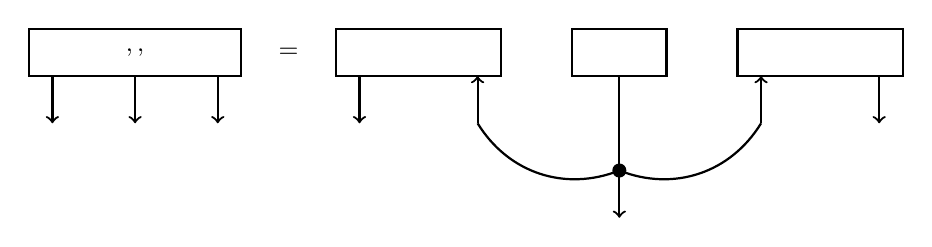
\begin{tikzpicture}[scale=0.3,thick] % , baseline = -3.5pt


\draw (-2,1) rectangle (7,-1);
\node[anchor=center] (text) at (2.5,0) {\small $\probof{\exrandom,\secexrandom,\thirdexrandom}$};
\draw[->] (-1,-1) -- (-1,-3) node[midway, left] {\tiny $\exrandom$};
\draw[->] (2.5,-1) -- (2.5,-3) node[midway, left] {\tiny $\secexrandom$};
\draw[->] (6,-1) -- (6,-3) node[midway, left] {\tiny $\thirdexrandom$};

\node[anchor=center] (text) at (9,0) {\small ${=}$};

\draw (11,1) rectangle (18,-1);
\node[anchor=center] (text) at (14.5,0) {\small $\condprobof{\exrandom}{\thirdexrandom}$};
\draw[->] (12,-1) -- (12,-3) node[midway, left] {\tiny $\exrandom$};
\draw[<-] (17,-1) -- (17,-3) node[midway, left] {\tiny $\thirdexrandom$};

\draw (21,1) rectangle (25,-1);
\node[anchor=center] (text) at (23,0) {\small $\probof{\thirdexrandom}$};
\draw (23,-1) -- (23,-3) node[midway, left] {\tiny $\thirdexrandom$};

\draw (23,-3) -- (23,-5);
\draw[fill] (23,-5) circle (0.25cm);
\draw[->] (23,-5) -- (23,-7) node[midway, left] {\tiny $\thirdexrandom$};
\draw (17,-3) to[bend right=40] (23,-5);
\draw (29,-3) to[bend right=-40] (23,-5);


\draw (28,1) rectangle (35,-1);
\node[anchor=center] (text) at (31.5,0) {\small $\condprobof{\secexrandom}{\thirdexrandom}$};
\draw[<-] (29,-1) -- (29,-3) node[midway, left] {\tiny $\thirdexrandom$};
\draw[->] (34,-1) -- (34,-3) node[midway, left] {\tiny $\secexrandom$};



\end{tikzpicture} 
\end{center}

\end{frame}





\section{Probability Decomposition}

\begin{frame}{Chain Rule: Decomposing Probabilities}

\begin{theorem}[Chain Rule]\label{the:chainRule}
	For any joint probability distribution $\probtensor$ of the variables $\probof{\catvariableof{0},\ldots,\catvariableof{\atomorder-1}}$ we have
	\begin{align*}
		\probtensor = \contractionof{\{\condprobof{\catvariableof{\atomenumerator}}{\catvariableof{0},\ldots,\catvariableof{\atomenumerator-1}}\, : \, \atomenumeratorin \}}{\{\enumeratedatoms\}}
	\end{align*}
	where for $\atomenumerator=1$ we denote by $ \condprobof{\catvariableof{0}}{\catvariableof{0},\ldots,\catvariableof{-1}}$ the marginal distribution $\probof{\catvariableof{0}}$.
\end{theorem}

\end{frame}


\begin{frame}{Markov Chains}

\begin{theorem}[Markov Chain]\label{the:MarkovChain}
	Let there be a set of variables $\catvariableof{\tenumerator}$ where $\tenumeratorin$.
	When $\catvariableof{\tenumerator}$ is independent of $\catvariableof{0:{\tenumerator-2}}$ conditioned on $\catvariableof{\tenumerator-1}$ (the Markov Property), then
	\begin{align*}
		\probtensor = \contractionof{\condprobof{\catvariableof{\tenumerator}}{\catvariableof{\tenumerator-1}}\, : \, \tenumeratorin}{
		\catvariableof{0},\ldots,\catvariableof{\tdim-1}
		} \, . 
	\end{align*}	
\end{theorem}

We depict this by 
\begin{center}
	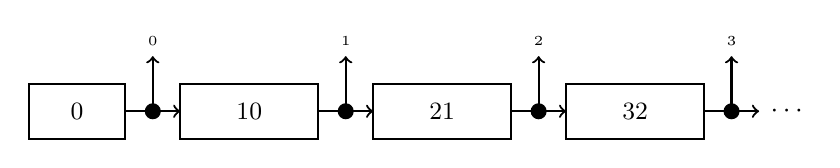
\begin{tikzpicture}[scale=0.35,thick] % , baseline = -3.5pt


\draw (-3.5,-1) rectangle (0, 1);
\node[anchor=center] (text) at (-1.75,0) {\small $\probof{\catvariableof{0}}$};
\draw[->] (0,0) -- (2,0);
\draw[fill] (1,0) circle (0.25cm);
\draw[->] (1,0) -- (1,2) node[above] {\tiny $\catvariableof{0}$};
\draw (2,-1) rectangle (7, 1);
\node[anchor=center] (text) at (4.5,0) {\small $\condprobof{\catvariableof{1}}{\catvariableof{0}}$};
\draw[->]  (7,0) -- (9,0);
\draw[fill] (8,0) circle (0.25cm);
\draw[->] (8,0) -- (8,2) node[above] {\tiny $\catvariableof{1}$};
\draw (9,-1) rectangle (14, 1);
\node[anchor=center] (text) at (11.5,0) {\small $\condprobof{\catvariableof{2}}{\catvariableof{1}}$};
\draw[->]  (14,0) -- (16,0);
\draw[fill] (15,0) circle (0.25cm);
\draw[->] (15,0) -- (15,2) node[above] {\tiny $\catvariableof{2}$};
\draw (16,-1) rectangle (21, 1);
\node[anchor=center] (text) at (18.5,0) {\small $\condprobof{\catvariableof{3}}{\catvariableof{2}}$};
\draw[->]  (21,0) -- (23,0);
\draw[fill] (22,0) circle (0.25cm);
\draw[->] (22,0) -- (22,2) node[above] {\tiny $\catvariableof{3}$};
\node[anchor=center] (text) at (24,0) {$\cdots$};

\end{tikzpicture} 
\end{center}


\end{frame}




\section{Hidden Markov Models}


\begin{frame}{Hidden Markov Models}

Hidden Markov Models extend Markov Chains by limited observation $\randomeof{\tenumerator}$ of the variables $\catvariableof{\tenumerator}$. \\
\medskip 
The independence assumptions are 
\begin{itemize}
	\item $\catvariableof{\tenumerator+1}$ is independent of $\catvariableof{0:\tenumerator-1}$ and $\randomeof{0:\tenumerator}$ conditioned on $\catvariableof{\tenumerator}$
	\item $\randomeof{\tenumerator}$ is independent of all other variables conditioned on $\catvariableof{\tenumerator}$
\end{itemize}
\medskip 
The independence assumptions are exploited in the decomposition
\begin{center}
	\begin{tikzpicture}[scale=0.3,thick] % , baseline = -3.5pt

    \node[anchor=center] (text) at (-1,3) {${a)}$};

    \node [circle, draw, thick, fill=\nodegrayscale, minimum size = \nodeminsize] (T1) at (0,0) {\colorlabelsize $\catvariableof{0}$};
    \node [circle, draw, thick, fill=\nodegrayscale, minimum size = \nodeminsize] (E1) at (0,-4) {\colorlabelsize $\randomeof{0}$};
    \draw[->-] (T1) -- (E1);
    \node [circle, draw, thick, fill=\nodegrayscale, minimum size = \nodeminsize] (T2) at (4,0) {\colorlabelsize $\catvariableof{1}$};
    \node [circle, draw, thick, fill=\nodegrayscale, minimum size = \nodeminsize] (E2) at (4,-4) {\colorlabelsize $\randomeof{1}$};
    \draw[->-] (T2) -- (E2);
    \draw[->-] (T1) -- (T2);
    \node [circle, draw, thick, fill=\nodegrayscale, minimum size = \nodeminsize] (T3) at (8,0) {\colorlabelsize $\catvariableof{2}$};
    \node [circle, draw, thick, fill=\nodegrayscale, minimum size = \nodeminsize] (E3) at (8,-4) {\colorlabelsize $\randomeof{2}$};
    \draw[->-] (T3) -- (E3);
    \draw[->-] (T2) -- (T3);
    \node [circle, draw, thick, fill=\nodegrayscale, minimum size = \nodeminsize] (T4) at (12,0) {\colorlabelsize $\catvariableof{3}$};
    \node [circle, draw, thick, fill=\nodegrayscale, minimum size = \nodeminsize] (E4) at (12,-4) {\colorlabelsize $\randomeof{3}$};
    \draw[->-] (T4) -- (E4);
    \draw[->-] (T3) -- (T4);
    \draw[->-] (T4) -- (15,0);

    \node[anchor=center] (text) at (16,0) {$\cdots$};

    %\node [circle, draw, thick, fill=\nodegrayscale, minimum size = \nodeminsize] (T4) at (17,0) {\colorlabelsize $\catvariableof{\atomorder}$};
    %\draw[->-] (14,0) -- (T4);


    \begin{scope}
        [shift={(22,0)}]

        \node[anchor=center] (text) at (-3,3) {${b)}$};

        \draw (-3.5,-1) rectangle (0, 1);
        \node[anchor=center] (text) at (-1.75,0) {\corelabelsize $\probat{\catvariableof{0}}$};
        \draw[->-] (0,0) -- (1.5,0);
        \draw[->-] (1.5,0) -- (2,0);
        \draw[fill] (1,0) circle (\dotsize);
        \draw (1,0) -- (1,2) node[above] {\colorlabelsize ${\catvariableof{0}}$};
        \draw[->-] (1,0) -- (1,-2);
        \draw (-1.5,-2) rectangle (3.5,-4);
        \node[anchor=center] (text) at (1,-3) {\corelabelsize $\condprobof{\randomeof{0}}{\catvariableof{0}}$};
        \draw[->-] (1,-4) -- (1,-6) node[midway, right]{\colorlabelsize ${\randomeof{0}}$};

        \draw (2,-1) rectangle (7, 1);
        \node[anchor=center] (text) at (4.5,0) {\corelabelsize $\condprobof{\catvariableof{1}}{\catvariableof{0}}$};
        \draw[->-]  (7,0) -- (8.5,0);
        \draw[->-]  (8.5,0) -- (9,0);
        \draw[fill] (8,0) circle (\dotsize);
        \draw (8,0) -- (8,2) node[above] {\colorlabelsize ${\catvariableof{1}}$};
        \draw[->-] (8,0) -- (8,-2);
        \draw (5.5,-2) rectangle (10.5,-4);
        \node[anchor=center] (text) at (8,-3) {\corelabelsize $\condprobof{\randomeof{1}}{\catvariableof{1}}$};
        \draw[->-] (8,-4) -- (8,-6) node[midway, right]{\colorlabelsize ${\randomeof{1}}$};


        \draw (9,-1) rectangle (14, 1);
        \node[anchor=center] (text) at (11.5,0) {\corelabelsize $\condprobof{\catvariableof{2}}{\catvariableof{1}}$};
        \draw[->-]  (14,0) -- (15.5,0);
        \draw[->-]  (15.5,0) -- (16,0);
        \draw[fill] (15,0) circle (\dotsize);
        \draw (15,0) -- (15,2) node[above] {\colorlabelsize ${\catvariableof{2}}$};
        \draw[->-] (15,0) -- (15,-2);
        \draw (12.5,-2) rectangle (17.5,-4);
        \node[anchor=center] (text) at (15,-3) {\corelabelsize $\condprobof{\randomeof{2}}{\catvariableof{2}}$};
        \draw[->-] (15,-4) -- (15,-6) node[midway, right]{\colorlabelsize ${\randomeof{2}}$};

        \draw (16,-1) rectangle (21, 1);
        \node[anchor=center] (text) at (18.5,0) {\corelabelsize $\condprobof{\catvariableof{3}}{\catvariableof{2}}$};
        \draw[->-]  (21,0) -- (22.5,0);
        \draw  (22.5,0) -- (23,0);
        \draw[fill] (22,0) circle (\dotsize);
        \draw (22,0) -- (22,2) node[above] {\colorlabelsize ${\catvariableof{3}}$};
        \draw[->-] (22,0) -- (22,-2);
        \draw (19.5,-2) rectangle (24.5,-4);
        \node[anchor=center] (text) at (22,-3) {\corelabelsize $\condprobof{\randomeof{3}}{\catvariableof{3}}$};
        \draw[->-] (22,-4) -- (22,-6) node[midway, right]{\colorlabelsize ${\randomeof{3}}$};


        \node[anchor=center] (text) at (24,0) {$\cdots$};


    \end{scope}

\end{tikzpicture} 
\end{center}

\end{frame}



\begin{frame}{Directed Graphical Models: Bayesian Networks}

\begin{definition}[Bayesian Networks]
	Let $\graph=(\nodes,\edges)$ be a directed acyclic graph and for each node $\node\in\nodes$ a random variable $\catvariableof{\node}$.
	Further let there be for each node $\node\in\nodes$ with parents $\parentsof{\node}$ a conditional probability distribution
		\[ \condprobof{\catvariableof{\node}}{\catvariableof{\parentsof{\node}}} \, . \]
	Then the \emph{Bayesian Network} with respect to $\graph$ and the conditional probability terms is the distribution
	\begin{align*}
		\probtensor = \contractionof{\condprobof{\catvariableof{\node}}{\catvariableof{\parentsof{\node}}} \, : \, \nodein}{\catvariableof{\node} \, : \, \nodein} \, .
	\end{align*}
\end{definition}

\end{frame}



\begin{frame}{Directed Graphical Models:\\ 
Bayesian Networks}

For each variable we build the conditional probability tensor
\begin{center}
	\begin{tikzpicture}[scale=0.35,thick] % , baseline = -3.5pt

\draw[->] (4.5,-1) -- (4.5,1) node[midway, right]{\tiny $\catvariableof{\node}$};
\draw (0,-1) rectangle (9,-4); 
\node[anchor=center] (text) at (4.5,-2.5) {\small $\condprobof{\catvariableof{\node}}{\catvariableof{\parentsof{\node}}} $};
\draw[->] (1,-6) -- (1,-4) node[midway, right]{\tiny $\catvariableof{0}$};
\draw[->] (2.5,-6) -- (2.5,-4) node[midway, right]{\tiny $\catvariableof{1}$};

\node[anchor=center] (text) at (5.5,-5) {$\cdots$};
	
\draw[->] (8,-6) -- (8,-4) node[midway, right]{\tiny $\catvariableof{\cardof{\parentsof{\node}}\shortminus1}$};



\end{tikzpicture} 
\end{center}
The \emph{Bayesian Network} is then the contraction
	\begin{align*}
		\probtensor = \contractionof{\condprobof{\catvariableof{\node}}{\catvariableof{\parentsof{\node}}} \, : \, \nodein}{\catvariableof{\node} \, : \, \nodein} \, .
	\end{align*}

\end{frame}



\begin{frame}{Undirected Graphical Models:\\  
Markov Networks}


\begin{definition}[Markov Networks]
	Let $\tnetof{\graph}$ be a Tensor Network on a hypergraph $\graph$.
	The associated Markov Network is the probability distribution of $\{\catvariableof{\node}\,:\,\nodein\}$ defined by 
		\[ \probtensorof{\graph} = \frac{
			\contractionof{\{\hypercoreof{\edge} : \edge \in \edges\}}{\nodes} 
		}{
			\contractionof{\{\hypercoreof{\edge} : \edge \in \edges\}}{\varnothing}
		} = \normalizationofwrt{\{\hypercoreof{\edge} : \edge \in \edges\}}{\nodes}{\varnothing} \, . \]
	We call the denominator
		\[\partitionfunctionof{\graph} = \contractionof{\{\hypercoreof{\edge} : \edge \in \edges\}}{\varnothing} \]
	the \emph{partition function} of the Markov Network.
\end{definition}

\end{frame}




\end{document}








\begin{frame}{Naive Bayes Classifier}

Causes and effects: Independence of causes conditioned on effect.

\end{frame}


\begin{frame}{Markov Chain}

Independence of history conditioned on previous state.

\end{frame}

